\section{Implementation med event sourcing}
Event sourcing er implementeret for bedre at adskille read og write modellen. Samt opnå eventual consistency.
Domæne delen er fjernet. Dvs. der ikke længere er gemt nogen entities. Tilgængel gemmes alle commands.
For at lave en entity må en read model selv skabe den, ved at kombinere alle relevante commands.
I dette projekt er defineret fire commands: AddUser, RenameUser, AddGroup og JoinGroup.
\begin{figure}[H]
	\center
	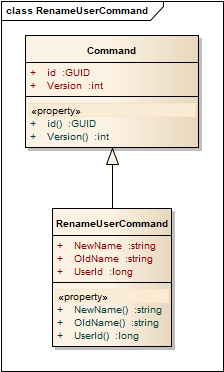
\includegraphics[width=0.25\textwidth]{RenameUserCommand.png}
	\caption{Eksempel på RenameUserCommand}
	\label{fig:RenameUserCommandl}
\end{figure}
Dette betyder f.eks. at en read model som gerne vil have alle brugere med navn. Bliver nød til at kombinere én AddUser command med alle tilhørende RenameUser commands.
En read model som er interesseret i grupper. Kunne nøjes med at kigge på AddGroup. Men hvis read modellen også er interesseret i gruppens medlemmer. Skal alle tilhørende JoinGroup commands gennemgås.
\begin{figure}[H]
	\center
	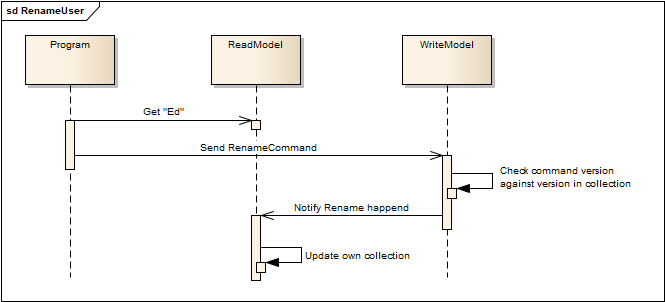
\includegraphics[width=1.0\textwidth]{RenameUserSimple.png}
	\caption{Sekvensdiagram der viser hvordan et program kan ændre navnet på en bruger}
	\label{fig:RenameUserSequence}
\end{figure}
På \ref{fig:RenameUserSequence} ses hvordan en bruger får skiftet sit navn. Der ses også at både read og write siden har en database.
Write siden har ikke nogen idé om hvad en User er. Den kender kun til RenameUser commanden.
Sekvensen er implementeret med de følgende tre metoder. 
\lstinputlisting[language=C]{Kode/RenameUserHandler.cs}
Denne handler ligger i Handlers.cs og er interfacet for write modellen. 
For at opnå eventual consistency tjekkes versions nummeret på commanden, mod det højeste versions nummer i databasen.
\lstinputlisting[language=C]{Kode/CommandRepositoryValidation.cs}
Herefter kaldes et event, hvilket resultere i at read modellen også får den nye command.
\lstinputlisting[language=C]{Kode/ApplyRenameUser.cs}
Apply ligger i Queries.cs. Og repræsentere kernen af en hvilket som helst read model.
Hvis vores applikation allerede havde en database med en masse commands. \\
Skulle en read model kalde Apply metoden på alle commands sorteret korrekt efter version. \\
Read modellen gemmer også den seneste command i den lokale relevante entitet. Denne bruges senere når der skal sendes flere commands. \\
